%%
%% Author: dariochinelli
%% 2020-10-13
%%

\section{Teoria quanto-meccanica di Shrodinger}

Con questa teoria è possibile esprimere l'equazione che controlla l'evoluzione di una funzione d'onda.
Essa è una funzione delle coordinate spaziali e del tempo, avente il significato di un'ampiezza di probabilità.
Sostanzialmente costituisce il principio dell'ipotesi di De Broglie.

$$ \Psi(x,t) = \sin \biggl[ 2 \pi \biggl( \frac{x}{\lambda} - \nu t \biggr) \biggr] $$

Questa è l'espressione del moto di una particella libera, cioè con $p=h/\lambda $ costante.

Tuttavia essa è troppo semplice e occorre cercare un'equazione più complicata, che soddisfi le seguenti:

\begin{enumerate}
\item deve essere consistente con $\lambda = h / p$ e $\nu = E / h$
\item deve essere consistente con $E = \frac{p^2}{2m} + V$
\item ogni combinazione lineare di soluzioni deve essere anch'essa soluzione.
\end{enumerate}

Nel 1925 Shrodinger formulò:

$$ -\frac{\hbar^2}{2m} \frac{\partial^2 \Psi(x,t)}{\partial x^2} + V(x,t) \Psi(x,t) = i \hbar \frac{\partial \Psi(x,t)}{\partial t} $$

Da cui si vede subito che nel caso di particella libera la soluzione dovrà appartenere al campo complesso.

$$ \Psi (x,t) = \cos(kx-\omega t) + i \sin(kx - \omega t) $$
con $k = \frac{2\pi}{\lambda}$

Si può quindi definire $P(x,t)$ che esprime la probabilità di trovare una particella in $x$ e $t$ dati, come:

$$ P(x,t) = \Psi^{\ast}(x,t)\Psi(x,t) = |\Psi(x,t)|^2 $$

L'equazione di Shrodinger dipende da $x$ e $t$ ma si può risolvere mediante la tecnica di separazione delle variabili, se il potenziale non dipende dal tempo.

$$ \Psi(x,t) = \Psi(x)\varphi(t) $$

$$ -\frac{\hbar^2}{2m} \frac{d^2}{dx^2} \Psi(x) + V(x)\Psi(x) = E\Psi(x) $$

$$E = \frac{p^2}{2m} + V = \frac{\hbar^2 k^2}{2m} + V \Rightarrow k^2 = \frac{2m}{\hbar^2}(E-V) $$

$$ \frac{d \varphi(t)}{dt} = - \frac{i E}{\hbar} \varphi(t) \Rightarrow \varphi(t) = e^{-i \frac{E}{\hbar} t} $$ \\


\textbf{Esempio:} \textit{particella libera, cerchiamo la funzione d'onda}

$$ \Psi(x) = \sin (\frac{2\pi x}{\lambda} = \sin(k x)) $$

$$ \frac{d\Psi}{dx} = k \cos(k x)$$

$$ \frac{d^2\Psi}{dx^2} = -k^2 \sin(k x)$$

$$ \frac{d^2\Psi}{dx^2} = - \frac{2m}{\hbar ^2} (E - V) \Psi(x) \Rightarrow - \frac{\hbar ^2}{2m} \frac{d^2 \Psi(x)}{dx ^2} + V(x)\Psi = E \Psi(x) $$

Abbiamo qui considerato il caso in cui $V = const$, ma si suppone che non cambi per $V=V(x)$.
Consideriamo ora $V=0$, in tal caso la soluzione generale è

$$ \Psi(x, t) = \Psi(x) e^{-\frac{i E t}{\hbar}} $$

dove $ k = \frac{2 \pi}{\lambda} $ e $ \omega = \frac{E}{\hbar} $

$$ \Psi(x, t) = \cos ( k x -\omega t ) + i \sin ( k x -\omega t ) = e^{ i (- k x - \omega t )} = e^{- i k x} e^{- i \omega t} $$

$$ \Psi (x) = e^{- i k x} \mbox{  e  }  \psi (t) = e^{- i \omega t} $$
è quindi soluzione anche una combinazione lineare di soluzioni 
$$\Psi (x) = A e^{i k x} + B e^{- i k x} $$.

Si ha un'\textbf{onda stazionaria} se $|A| = |B| $. \\

\textbf{Esempio:} \textit{buca di potenziale infinita}

\begin{figure}[h]
\centering
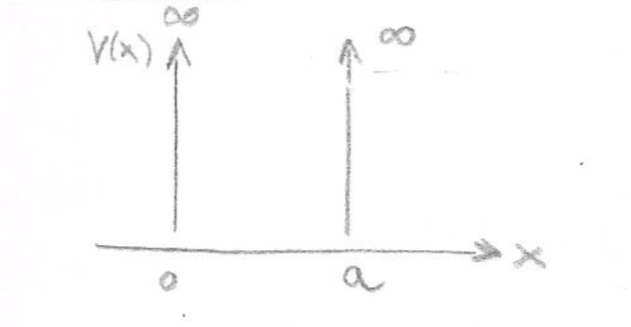
\includegraphics[scale=0.3]{/potenziale_buca_infinita}
\end{figure}

Nella regione esterna non c'è probabilità di trovare la particella $\Rightarrow \Psi (x) = 0$, mentre all'interno è come per la particella libera, 
e quindi $\Psi (x) = A e^{i k x} + B e^{- i k x} $

\begin{equation}
V(x) = 
\begin{cases}
	\infty \Longleftrightarrow x>a \vee x<0 \\
	0 \Longleftrightarrow 0 < x < a
\end{cases}
\end{equation}

Quest'onda dovrà perciò avere due poli fissi in $0$ e $a$.

$$\Psi (x) = A ( e^{i k x} - e^{- i k x} ) = 2 i A \sin(k x) = c \sin(k x) $$

\begin{equation}
\begin{cases}
	\Psi(0) = A + B = 0 \Rightarrow B = - A \\
	\Psi(a) = c \sin(k a) = 0 \Rightarrow k a = n \pi \mbox{ con } n \in Z
\end{cases}
\end{equation}

$$ \Rightarrow k = \frac{n \pi}{a} \Rightarrow p = \frac{n \pi \hbar}{a} \iff \mbox{ La quantità di moto è quantizzata!} $$

$$ E = \frac{p^2}{2m} = \frac{\hbar k^2}{2m} = \frac{n^2 \pi^2 \hbar^2}{2 m a^2} \iff \mbox{ L'energia è quantizzata!} $$

$$ \Psi_{n} (x) = c \sin \bigl( \frac{ n \pi x }{a} \bigr) $$



Il minimo dell'energia non è dunque zero bensì $E_1 = \frac{\hbar^2 \pi^2}{2 m a^2} $

\begin{equation}
\begin{cases}
	\Delta x = a \\
	\Delta p \geq \frac{\hbar}{2a}
\end{cases}
\end{equation}

Ogni particella confinata ha energia minima diversa da zero come conseguenza del Principio di Indeterminazione. \\

\textbf{Esempio:} \textit{scatola tridimensionale}

\begin{equation}
\begin{cases}
	p_x = \frac{\pi \hbar n_x}{a} \\
	p_x = \frac{\pi \hbar n_y}{b} \\
	p_x = \frac{\pi \hbar n_z}{c}
\end{cases}
\Longrightarrow E = \frac{p^2}{2m} = \frac{1}{2m} ( p_x^2 + p_y^2 + p_z^2 ) \\
= \frac{\pi^2 \hbar^2}{2m} (\frac{n_x^2}{a^2} + \frac{n_y^2}{b^2} + \frac{n_z^2}{c^2} )
\end{equation}

Se $a=b=c$ ed $a$ è il lato del cubo si ottiene:

$$ E = \frac{\pi^2 \hbar^2}{2 m a} r^2 $$

\begin{figure}[h]
\centering
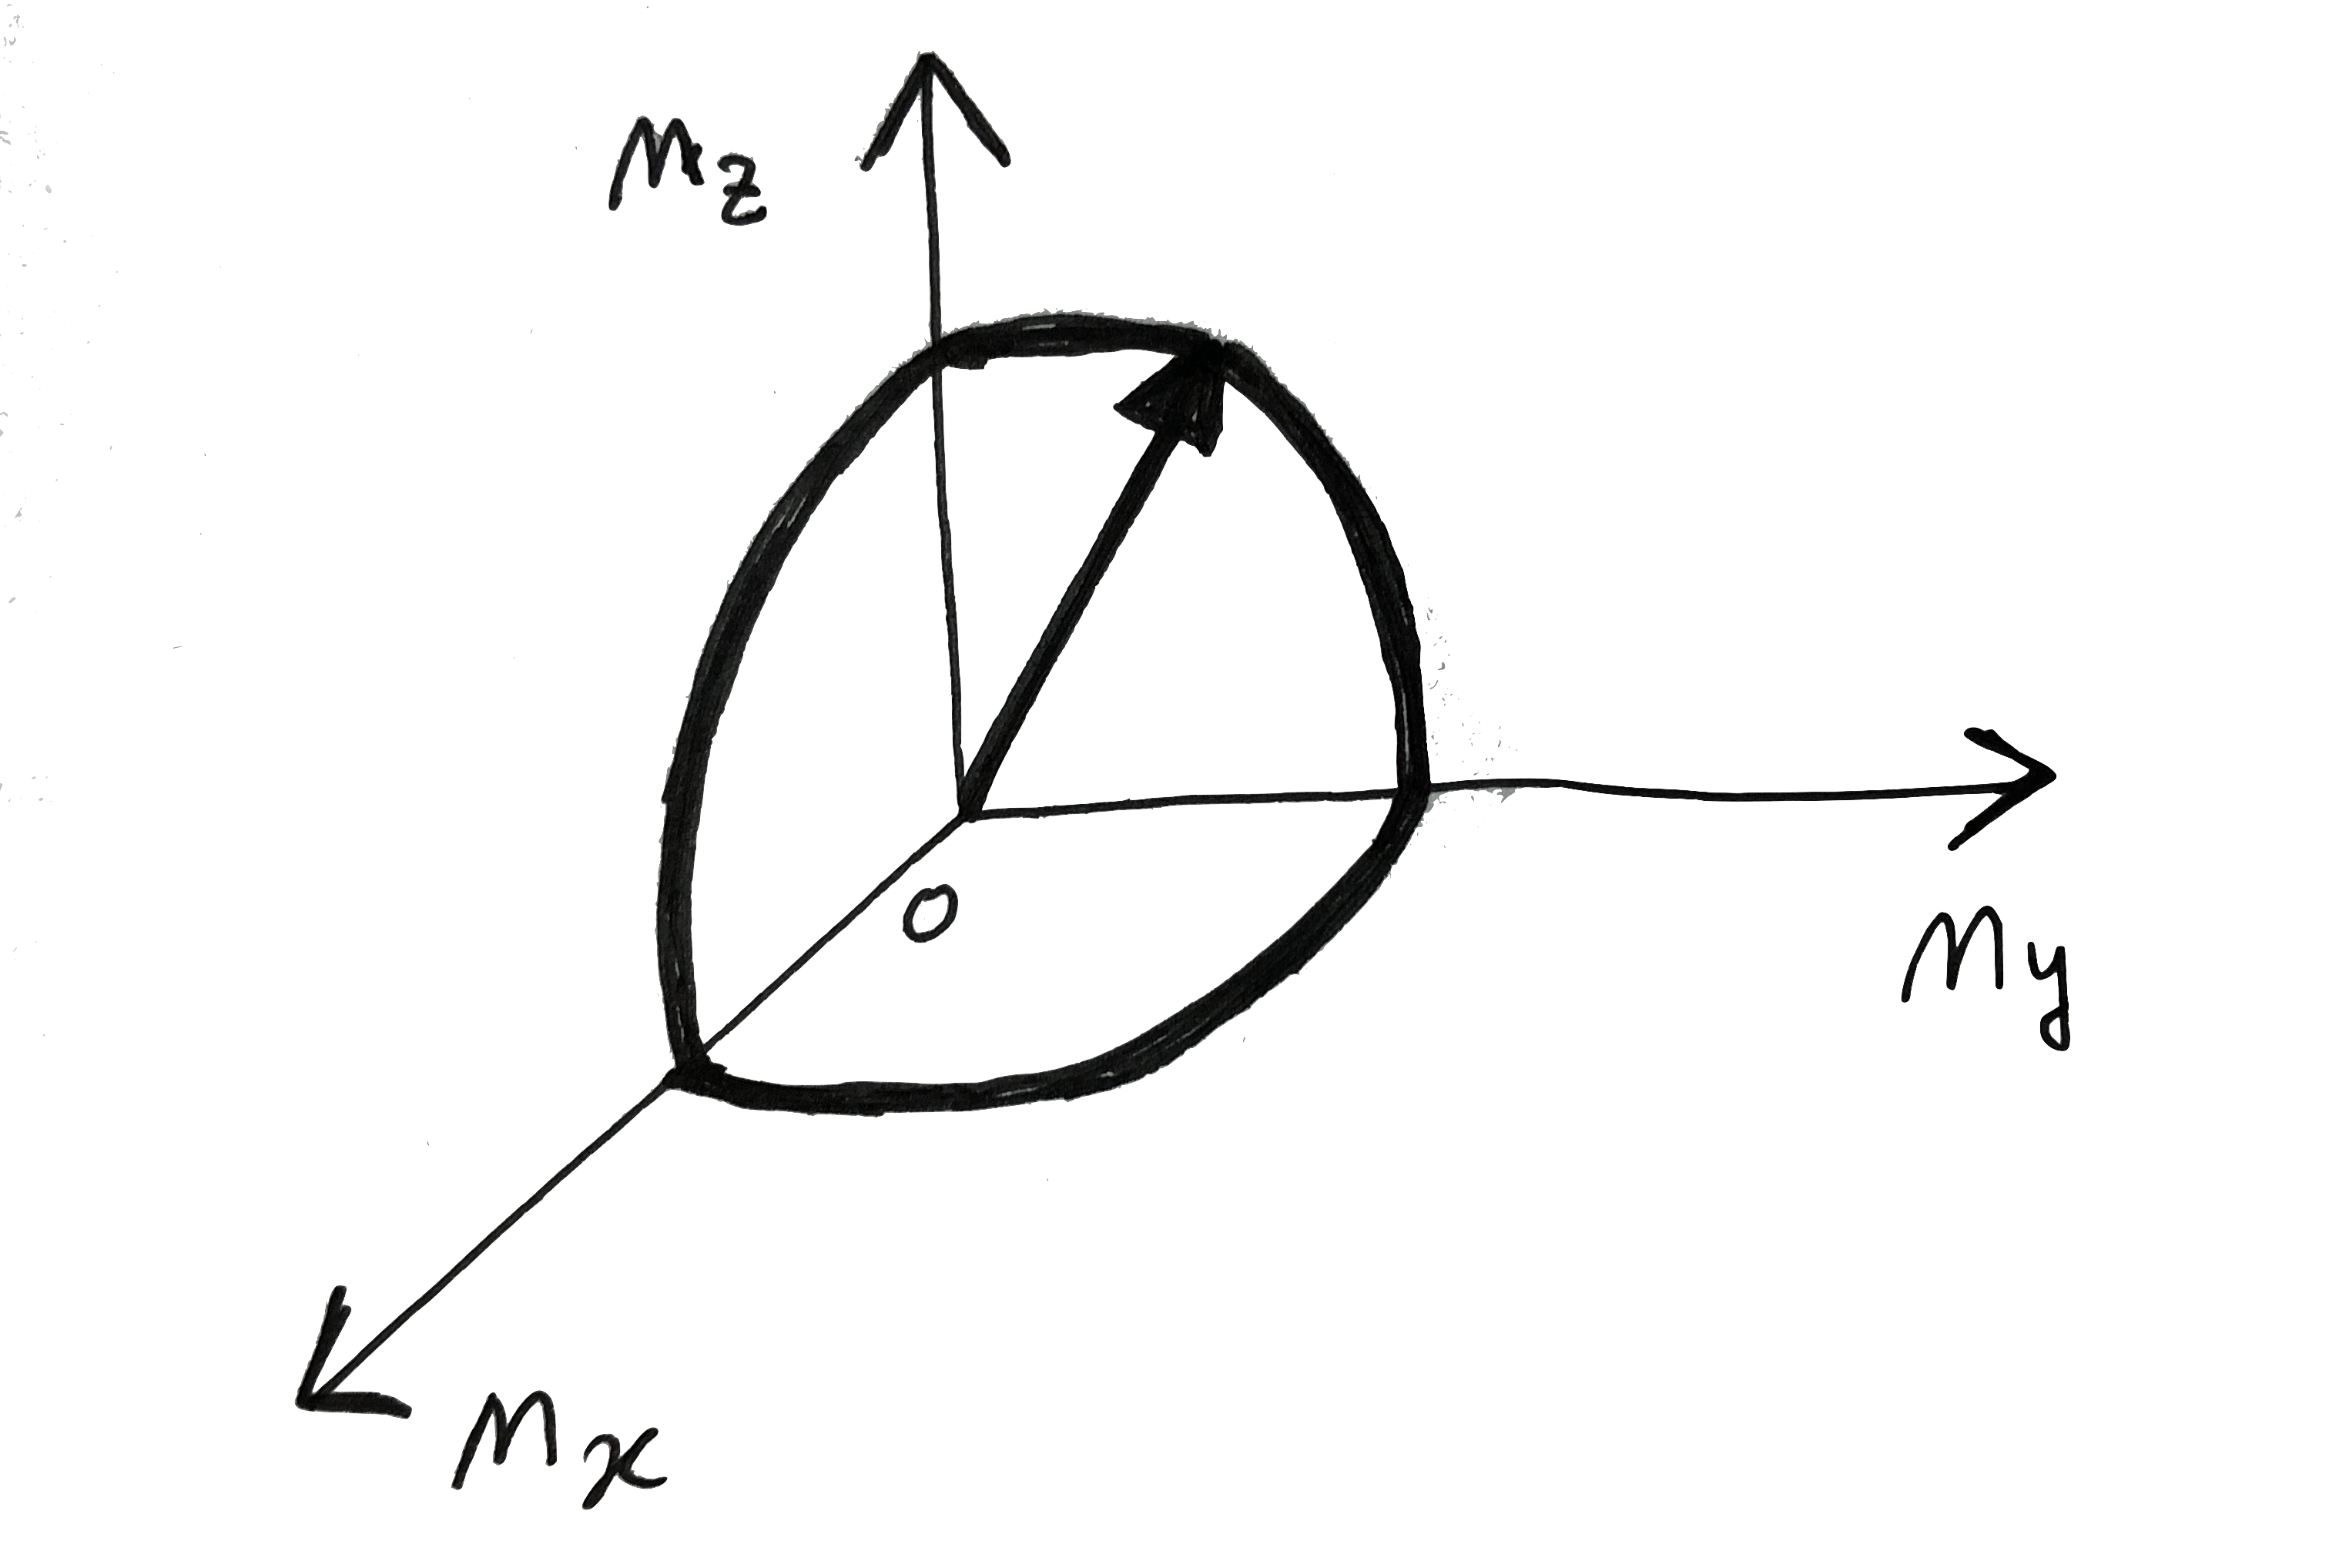
\includegraphics[scale=0.05]{/Energy_raggio}
\end{figure}

Se $a$ è piccolo i livelli energetici sono distanti, ma se $a$ è grande allora sono molto ravvicinati.

Cerco dunque una funzione "densità di livelli energetici" nell'intervallo da $E$ a $E+dE$.

Considero ogni punto $P$, che sta sulla superficie della sfera di raggio $r$, con uguale energia.
Numero di stati di energia compresi fra $0$ e $E$ 

$$ N(E) = \frac{1}{8} \Bigl( \frac{4}{3} \pi r^3 \Bigr) = \frac{\pi}{6} a^3 \Bigl( \frac{2 m E}{\pi^2 \hbar^2} \Bigr) ^{\frac{3}{2}} = 
\frac{8 \pi V}{3 \hbar^3} \Bigl(2 m^3 \Bigr) ^{\frac{1}{2}} E^{\frac{3}{2}} $$

Ma quanti ce ne sono in un $dE$? 

$$ dN(E) = \frac{4 r V}{\hbar^3} (2 m^3)^{\frac{1}{2}} E^{\frac{1}{2}} dE $$

Da qui si trova la \underline{funzione densità degli stati}

$$ \frac{dN}{dE} = g(E) = \frac{4 r V}{\hbar^3} (2 m^3)^{\frac{1}{2}} E^{\frac{1}{2}} $$

Che si può trovare anche in funzione di $p$, tale che 
$ g(p) dp = g(E) dE $ e $  \frac{dN}{dE} = g(p) = g(E)  \frac{dE}{dp} $

$$ g(p) = \frac{4 \pi V (2m^3)^\frac{1}{2}}{\hbar^3}  E\frac{1}{2} \frac{dE}{dp}$$

$$ \frac{dE}{dp} = \frac{p}{m}  \Longrightarrow g(p) = \frac{4 \pi V (2m^3)^{\frac{1}{2}}}{\hbar^3} \frac{p^2}{\sqrt{2m}} \frac{1}{m} = \frac{4 \pi V}{\hbar^3} p^2 $$

E poiché $ p = \frac{h}{\lambda} $ e $ \nu = \frac{c}{\lambda} $ e $ g(p) dp = g(\nu) d\nu $ si ha che

$$ g(\nu) = g(p) \frac{dp}{d\nu} = \frac{8 \pi V}{c^2} \nu^2 $$

formula di Planck per il Corpo Nero, dove il fattore 2 è dato dalla doppia polarizzazione.








